\documentclass[10pt]{article}
\usepackage[utf8]{inputenc}
\usepackage{cite}
\usepackage{url}
\usepackage[brazil]{babel}

\title{IF685 - Gerenciamento de Dados e Informação}
\author{Pedro Henrique Dias Monte de Freitas}
\date{Maio de 2019}

\usepackage{natbib}
\usepackage{graphicx}

\begin{document}

\maketitle

\section{Introdução}
Gerenciamento de Dados e Informação \cite{site}, disciplina ofertada no 4º período do curso de Ciência da Computação e que nos últimos períodos foi ministrada pela professora Valéria Times, tem como objetivo oferecer aos alunos conhecimento geral sobre Banco de Dados, sendo essa a grande área da computação que ela se insere. A disciplina está dividida em alguns tópicos, sendo os principais deles: Modelagem de Dados \cite{navathe}, Banco de Dados Relacionais \cite{ramak}, Banco de Dados Objeto-Relacionais, Linguagem de 4ª Geração - PL e Dados Semi-Estruturados.

\begin{figure}[h!]
\centering
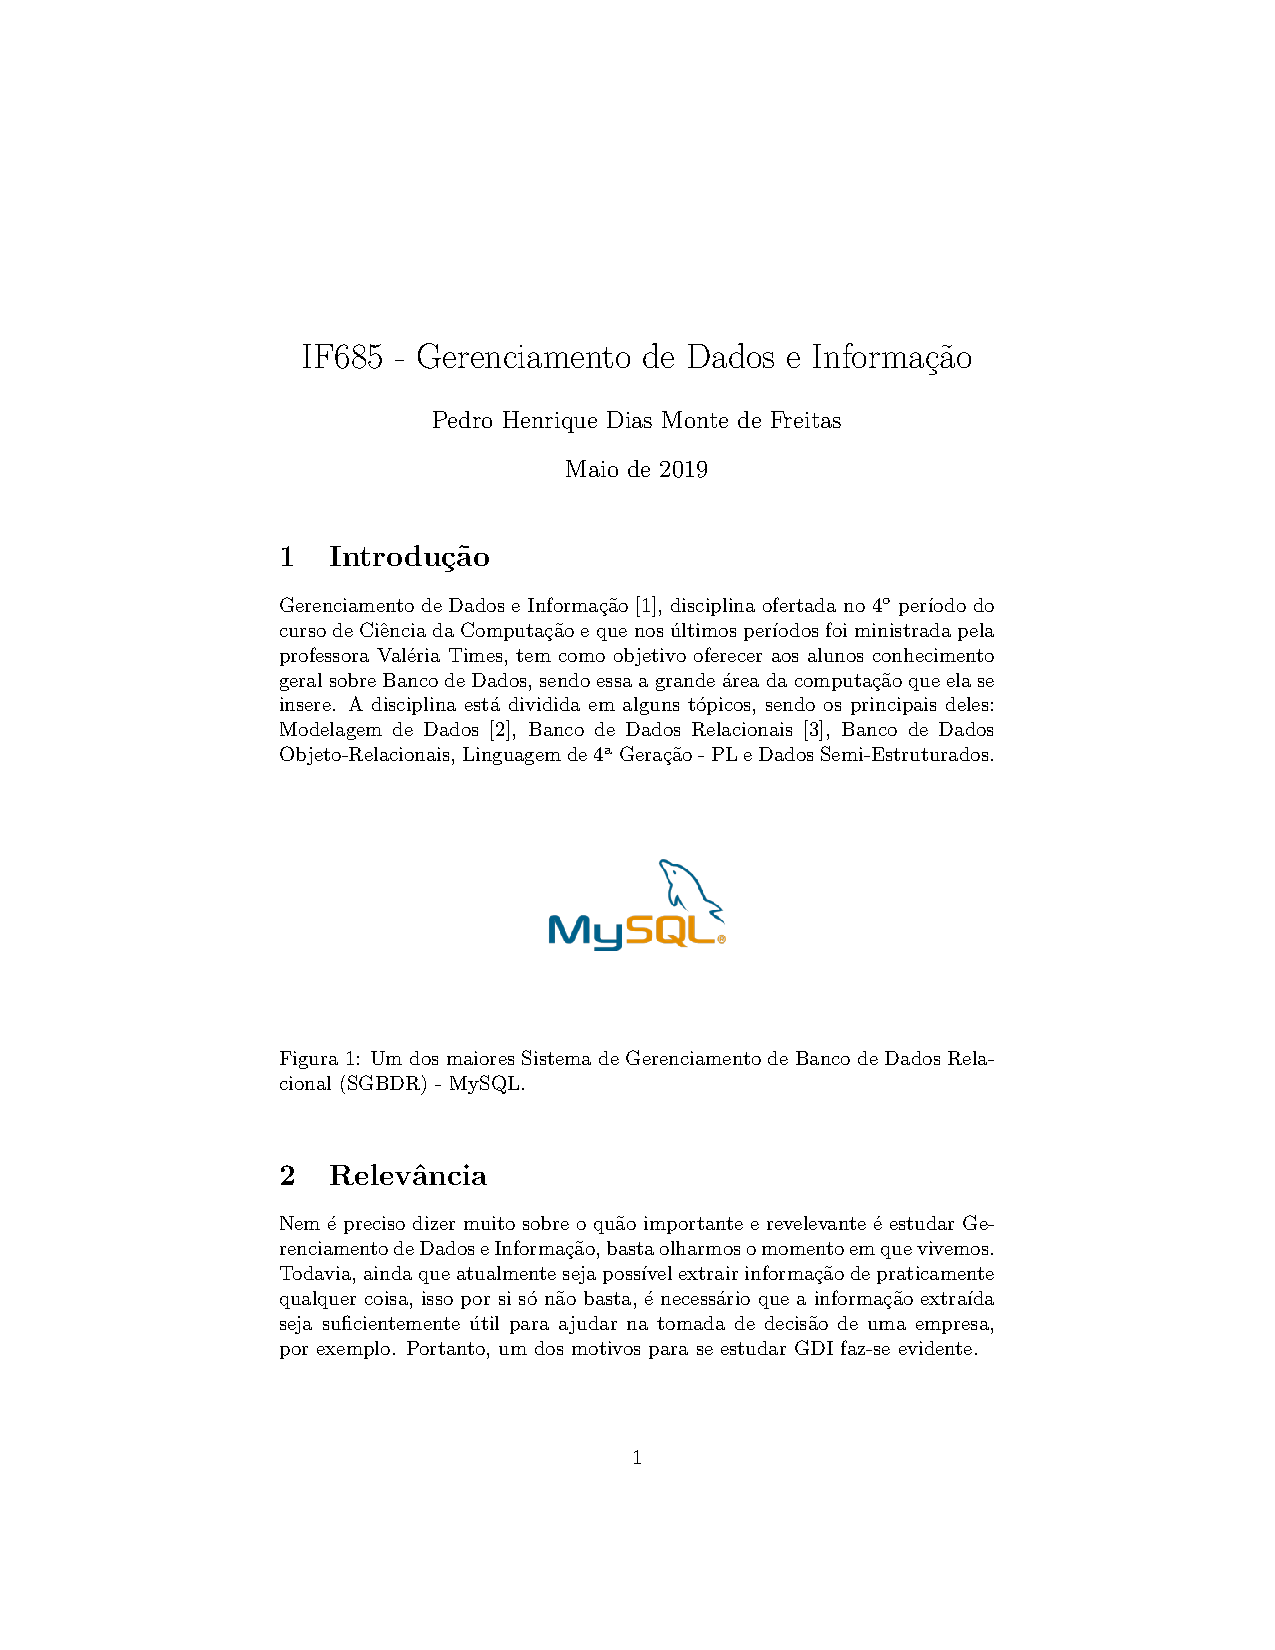
\includegraphics[scale=0.4]{phdmf.png}
\caption{Um dos maiores Sistema de Gerenciamento de Banco de Dados Relacional (SGBDR) - MySQL. \cite{img}}
\label{fig:phdmf}
\end{figure}

\section{Relevância}
Nem é preciso dizer muito sobre o quão importante e revelevante é estudar Gerenciamento de Dados e Informação, basta olharmos o momento em que vivemos. Todavia, ainda que atualmente seja possível extrair informação de praticamente qualquer coisa, isso por si só não basta, é necessário que a informação extraída seja suficientemente útil para ajudar na tomada de decisão de uma empresa, por exemplo. Portanto, um dos motivos para se estudar GDI faz-se evidente.

\subsection{Pontos Positivos e Pontos Negativos}
Pontos Positivos: mais de uma área relacionada a Dados é vista na disciplina e os alunos são instigados a colocar em prática o conhecimento adquirido por meio de trabalhos e listas de exercícios. Em contrapartida, como ponto negativo vale ressaltar que, embora sejam feitos muitos exercícios e trabalhos, falta um projeto maior envolvendo apenas Banco de Dados, tal como o que acontece na cadeira de Introdução à Programação.  


\section{Relação com outras disciplinas}

\begin{table}[h]
 \centering
 {\renewcommand\arraystretch{1.25}
 \begin{tabular}{ l l }
  \cline{1-1}\cline{2-2}  
    \multicolumn{1}{|p{3cm}|}{Disciplina \centering } &
    \multicolumn{1}{p{6cm}|}{Relação \centering }
  \\ 
  \cline{1-1}\cline{2-2}  
    \multicolumn{1}{|p{3cm}|}{IF693 -  Sistema de Gerenciamento de Banco de Dados \centering } &
    \multicolumn{1}{p{6cm}|}{É possível dizer que GDI tem um foco maior na área de Dados, isto é, apresentar o máximo possível da área, no entanto, a disciplina de SGBD tem como objetivo estudar de forma aprofundada SGBDs, ou seja, desde uma visão mais geral até técnicas mais específicas.}
  \\ 
  \cline{1-1}\cline{2-2}  
    \multicolumn{1}{|p{3cm}|}{IF694 - Banco de Dados Distribuídos e Móveis \centering } &
    \multicolumn{1}{p{6cm}|}{Nesse caso, GDI serve como base em banco de dados, já que em BDDM são vistos conceitos fundamentais de bancos de dados distribuídos. Pode-se dizer que BDDM é uma parte específica da área de Banco de Dados, logo GDI é fundamental para o aluno que deseja aprender sobre.}
  \\
  \cline{1-1}\cline{2-2}  
    \multicolumn{1}{|p{3cm}|}{IF695 - Banco de Dados Avançados \centering } &
    \multicolumn{1}{p{6cm}|}{Assim como na disciplina anterior, GDI servirá de base para que o aluno esteja melhor contextualizado em relação a Banco de Dados.}
  \\ 
  \hline
\end{tabular}}
\end{table}

\bibliographystyle{plain}
\bibliography{phdmf}

\end{document}
